\documentclass[10pt,final,conference,comsoc]{IEEEtran}

% reviewer 1, comment 1 and 7 haven't been extended.
% Some figure maybe need to be fixed a little bit.
\usepackage[utf8]{inputenc}

\usepackage[T1]{fontenc} % optional
\usepackage{amsmath,amssymb,amsfonts}
\usepackage[cmintegrals]{newtxmath}
\usepackage{cite}
\usepackage{algorithmic}
\usepackage{graphicx}
\usepackage{textcomp}
\usepackage{xcolor}
\usepackage{bm}
\usepackage{siunitx}
\usepackage{comment}
\usepackage{mathtools}

\def\BibTeX{{\rm B\kern-.05em{\sc i\kern-.025em b}\kern-.08em
    T\kern-.1667em\lower.7ex\hbox{E}\kern-.125emX}}

\newcommand{\LRT}[2]{
  \mathrel{\mathop\gtrless\limits^{#1}_{#2}}
}
\newcommand{\numb}[1]{\SI{#1}}
\newcommand{\dB}{\decibel}
\newcommand{\est}[2]{\hat{#1}_{#2}}
\newcommand{\sd}{\text{SD}}
\newcommand{\cn}{\mathcal{CN}}
\newcommand{\n}{\mathcal{N}}
\newcommand{\opt}{\text{opt}}
\newcommand{\nm}{\text{NM}}
\newcommand{\J}{\mathrm{J}}
\newcommand{\prob}[1]{\text{P}_{#1}}
\newcommand{\fa}{\text{FA}}
\newcommand{\D}{\text{D}}
\newcommand{\E}{\mathbb{E}}
\newcommand{\Q}{\mathrm{Q}}
\newcommand{\Lagr}{\mathcal{L}}


\graphicspath{{../main_matlab_figures/}{../matlab/}}

\DeclareUnicodeCharacter{0303}{}

\begin{document}

\title{Low Complexity Methods for Joint Detection and Synchronization of TDMA Bursts
}

\author{\IEEEauthorblockN{Haotian Zhai 
  and Bernd-Peter Paris}
\IEEEauthorblockA{\textit{Department of Electrical and Computer Engineering} \\
\textit{George Mason University}\\
Fairfax, VA 22030 \\
\{hzhai,pparis\}@gmu.edu}
}

\maketitle


\begin{abstract}

This paper proposes a data-aided joint detection and synchronization algorithm for TDMA bursts.
A sequential detection algorithm based on the Generalized Likelihood Ratio Test (GLRT) is used to 
detect the embedded preamble signal in received data stream. 
% sequential detection algorithm is necessary to be derived.
Carrier synchronization is attempted for each sample instant during sequential detection and
resulting phase and frequency estimates are used by the GLRT. 
To make this algorithm implemented in software-defined radio (SDR),
a low complexity carrier estimation algorithm with good estimation accuracy is proposed.
Then, a refinement of the carrier estimate is computed when the preamble has been detected.
% SDR is also mentioned in abstract.
It is shown that this estimate approaches the Cramer-Rao bound even at low SNR. 
The complete joint detection and estimation procedure is validated through simulations and SDR.

\end{abstract}

\begin{IEEEkeywords}
Joint detection and estimation, GLRT, low computational complexity, Cramer-Rao vector bound, Software-defined radio.
\end{IEEEkeywords}

\section{Introduction}
\label{sec:introduction}

In digital communication systems, information is commonly transmitted in time-multiplexed bursts.
Examples include time-slotted random access systems. Each active user transmits in-formation to the receiver
in the same frequency band and in non-overlapping time intervals~\cite{Falconer_95}. 
A fundamental prerequisite for successful coherent demodulation is that the receiver can
detect the beginning of the data stream and estimate accurately the phase and frequency offset of the carrier.
It is worth empha-sizing that time and carrier synchronization are coupled prob-lems, especially at low SNRs:
coherent methods for detecting the signal require accurate frequency and phase estimates 
whi-le data-aided frequency and phase estimation requires that the location of the training sequence is available.
Thus, joint signal detection and carrier synchronization algorithms play a vital role in any communication system.

Clearly, the signal acquisition problem has been considered widely. 
In the late 90's, Morelli and Mengali~\cite{Morelli_Mengali_98} presented a tutorial review
of the carrier synchronization field comparing such characteristics as estimation accuracy, range,
and compu-tational complexity of available techniques. The work by~\cite{kay_89,Fitz_94,Luise_Reggiannini_95}
is most related to results in this paper. For signal detection,
particularly, sequential detection process, most of the sequential detector
is built based on hypothesis testing~\cite{Ramakrishnan_10,Chiani_06,Liang_15}.
More-over, the lack of information happens commonly when build
likelihood ratio test (LRT). For example, the LRT in~\cite{Chiani_06} 
is built based on the distribution of data stream, which is unknown.
The LRT is then replaced by generalized likelihood ratio test.

In this paper, we propose a joint detection and estimation algorithm 
for the signal acquisition process and implement it on software-defined radio (SDR).
In particular, the detection algorithm operates sequentially for every incoming sample
and is built based on the estimates from the carrier synchronization.
Thus, a family of low-complexity and high-accuracy estimators is proposed for implementing
in sequential detection and coherent demodulation on SDR at very high sample rate.


\section{Signal Model}
\label{sec:model}

\begin{figure}[t]
  \centerline{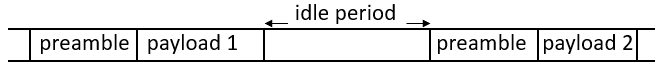
\includegraphics[width=3.4in]{data_structure.png}}
  \caption{Structure of signal stream at the receiver}
  \label{fig:data_structure}
  \end{figure}

In an uplink multiuser system, the transmitted signal frame from each user is seperated by an unkown length of idle period and assumed to include a reference signal that is known to the receiver.
Often such a reference sequence is prepended to the payload and is referred to as a preamble.
The structure of signal stream at the receiver is shown in Figure~\ref{fig:data_structure}. 
The problem addressed in this paper is to accurately estimate the start time of the preamble and to estimate carrier phase and frequency offset from the preamble.
Hence, the payload portion of the frame is not further considered. 
% Moreover, to make our algorithm applicable for signal transmission in very high speed,
% the complexity of algorithm is also crucial.

We now give the signal model for this paper. The received RF signal is first modulated at base band.
In~\cite{Morelli_Mengali_98} and~\cite{Ramakrishnan_10}, 
the authors obtain a simplifed signal model from the matched filter outputs by assuming the symbol time is perfectly known.
However, in practice, this is unreliable especially at low SNR. To accommodate this issue, we analyze the discrete signal model
directly after down-conversion and sampling, which yields received samples $r_n$

\begin{equation}
    \begin{aligned}
      \label{eq:model}
      r_n = s_{n-\bar{p}}Ae^{j\phi}e^{j2\pi\delta n}+w_{n},
    \end{aligned}
  \end{equation}
where $s_n$ denotes the sampled reference sequence (the preamble), which has the form

\begin{equation}
    \label{eq:l_ref_sig_discrete}
    s_n=\sum_{i=0}^{L_0-1} c_i g(nT_s-iT) \quad \text{for}~n=0,\ldots,N-1, 
    % \begin{dcases}
    %  \sum_{i=0}^{L_0-1} c_i g(nT_s-iT) & \text{for}~n=0,\ldots,N-1, \\
    %  0 & \text{otherwise}.
    % \end{dcases}
  \end{equation}
In~\eqref{eq:model}, $\bar{p}$ denotes the start position of the received preamble.
Note, because of the uncertainty of sampling, often the sampler may not sample exactly at the start time of the preamble, which causes
the integer delay $p$ with a fractional delay in the range of $[-\frac{T_s}{2},\frac{T_s}{2})$, where $T_s$ is the sample period as in~\eqref{eq:l_ref_sig_discrete}.
In this paper, the sampling rate is assumed to be high enough relative to the symbol rate, so that the influence of fractional delay can be ignored.
$A$, $\phi$, $\delta$ are the amplitude, carrier phase and normalized
frequency offset with respect to sample period $T_s$ that we want to estimate.
$w_n$ is complex AWGN. Moreover,
$E_s/N_0$ denotes the ratio of signal energy to noise power spec-tral density (SNR).
To make analysis easier, we assume a con-stant and normalized envelope of the samples in the 
preamble, i.e., $A^2|s_n|^2\approx A^2=E_s/M$ for $n=[0,N-1]$, where $M$ is the rate
of oversampling in each symbol of the preamble.

In~\eqref{eq:l_ref_sig_discrete}, $T$ denotes the symbol period and $g(t)$ provides pulse shaping.
$\{c_i\}_{i=0}^{L_0-1}$ is the symbol sequence known at transmitter and receiver, where $L_0$ denotes the number of symbols.
% We further define $M$ to be the rate of oversampling in each symbol, thus $M=\frac{T}{T_s}$, and 
We define $N=ML_0$ to be the number of samples in the preamble.
Note, compared with the signal model in~\cite{Morelli_Mengali_98} and~\cite{Ramakrishnan_10}, 
by using an oversampled signal, we can mitigate the coherent loss that occurs
when the signal with frequency offset is passed through the matched filter.
This allows our system to tolerate larger frequency offsets.

% Finally, note that in~\eqref{eq:l_ref_sig_discrete}, when the discrete time index $n$ of $s_n$ is greater than $N-1$,
% or equivalently, $n>p+N-1$ in~\eqref{eq:model}, it means the received samples $r_n$ at those $n$ are in the payload;
% We assume the data of payload is zero for simplicity (normally it isn't) because it does not affect the time synchronization of the preamble and carrier synchronization from the preamble.


% The rest of paper includes two main sections. The first section (Section 3 and 4) focus on 
% analyzing the signal acquisition chain, which includes the sequential detection process and
% carrier synchronization of the preamble. The above block diagram is shown in Figure 2.
% The simulation section 5 then illustrates the performance of proposed algorithm
% in the first section. The second section (section 6) moves attention on implementing the algorithm on software-defined radio (SDR).
% Some steps (equations) in the first section are computed more efficiently to achieve the best throughput.

\section{Detection and Time Synchronization}%
\label{sec:detection}

\begin{figure}[t]
  \centerline{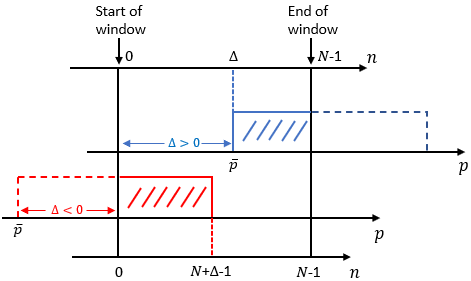
\includegraphics[width=2.75in]{partial_preamble_detection.png}}
  \caption{The current window with local time-scale $n$ may contain a
    partial preamble. The preamble starts at $\bar{p}$ on global scale.
    The start of the preamble relative to the window is $\Delta$. The cases $\Delta >0$ and $\Delta < 0$
    are illustrated.}
  \label{fig:partial_preamble_detection}
  \end{figure}

% In this section, we analyze the sequential detection problem, where 
% the detection algorithm proceeds sequentially and each step a window of
% $N$ received samples with $N{-}1$ overlapped samples from the previous window is considered.
We start by looking at the two hypotheses for the sequential detection task:
Let $H_0$ be the null hypothesis that the received signal is the
channel noise or only contains a portion of the preamble against the
alternative $H_1$ that it contains the entire preamble.  
% The detection algorithm proceeds sequentially and each step a window of
% length $N$ received samples with $N-1$ overlapped samples from the previous window is considered.
Define $\Delta$ to be the distance between the current start position of the window
of $N$ received samples and the start position of the preamble $\bar{p}$.
Fig.~\ref{fig:partial_preamble_detection} illustrates two distinct cases when a portion of the 
preamble is in the window.
%with global delay index $p$ and local sample index $n$.
In terms of the local scale $n=0,1,\ldots,N-1$, the two hypotheses are given by the window of samples $r_n$
\begin{equation}
  \label{eq:two hypotheses}
  \begin{aligned}
  &H_0{:}~r_n{=}
  \begin{dcases}
      s_{n-\Delta}\xi e^{j2\pi\delta (n-\Delta)}{+}w_n & \max(0{,}\Delta){\leq} n{<} \min(N{,}N{+}\Delta) \\
      % s_{n-\Delta}\xi e^{j2\pi\delta (n-\Delta)}{+}w_n & n{\in}[\max(0,\Delta), \min(N,N{+}\Delta)) \\
      w_n & \text{otherwise},
  \end{dcases} \\
  &H_1{:}~r_n{=}s_n\xi e^{j2\pi\delta n}+w_n.
  \end{aligned}
\end{equation}
where $\xi=Ae^{j\phi}$ denotes the phasor in~\eqref{eq:model}.
Furthermore, $\Delta \neq 0$ is the premise under hypothesis $H_0$
while $\Delta=0$ under $H_1$.  
% Figure 3 demonstrates the case when $H_0$ represents a portion of the preamble compared with
% $H_1$. 

We focus on discussing when the start of the preamble 
occurs in the window, i.e., $\Delta\in(0,N{-}1]$, which corresponds to
the top case in fig.~\ref{fig:partial_preamble_detection}.
The bottom case when 
$\Delta\in[-N{+}1,0)$ 
is symmetric to the top case.
Based on~\eqref{eq:two hypotheses}, we build conditional likelihood ratio test (CLRT)
between $H_0$ and $H_1$ by conditioning on the distance $\Delta$, 
the phasor $\xi$ and the frequency offset $\delta$. The conditional log likelihood ratio reduces to
% is given by
% \begin{equation}
%     \label{eq:likelihood ratio}
%     \begin{aligned}
%     \Lambda(R|\Delta,\xi,\delta)&=\frac{f_{R|H_1,\xi,\delta}(r|H_1,\xi,\delta)}{f_{R|H_0,\Delta,\xi,\delta}(r|H_1,\Delta,\xi,\delta)} \\
%     &=\frac{\displaystyle \prod_{n=0}^{N-1}\frac{1}{\sqrt{\pi N_0}}e^{-\frac{|r_n-s_n\xi e^{j2\pi\delta n}|^2}{N_0}}}{\displaystyle \frac{1}{(\pi N_0)^{N/2}}\prod_{n=\Delta}^{N-1}e^{-\frac{|r_n-s_{n-\Delta}\xi e^{j2\pi\delta (n-\Delta)}|^2}{N_0}}\prod_{n=0}^{\Delta-1}e^{-\frac{|r_n|^2}{N_0}}} \\
%     % &=\frac{\prod_{n=0}^{N-1}\frac{1}{\sqrt{\pi N_0}}e^{-\frac{|r_n-s_n\xi e^{j2\pi\delta n}|^2}{N_0}}}{\prod_{n=\Delta}^{N-1}\frac{1}{\sqrt{\pi N_0}}e^{-\frac{|r_n-s_{n-\Delta}\xi e^{j2\pi\delta (n-\Delta)}|^2}{N_0}}\prod_{n=0}^{\Delta-1}\frac{1}{\sqrt{\pi N_0}}e^{-\frac{|r_n|^2}{N_0}}} \\
%     % &\times \frac{1}{\prod_{n=0}^{\Delta-1}\frac{1}{\sqrt{\pi N_0}}e^{-\frac{|r_n|^2}{N_0}}}
%     & \LRT{H_1}{H_0} \eta.
%     \end{aligned}
%   \end{equation}
  % Canceling the common parts and taking the logarithm,~\eqref{eq:likelihood ratio} is reduced to
\begin{equation}
    \label{eq:log likelihood}
    \begin{aligned}
    \Re\Bigg\{\sum_{n=0}^{N-1}r_ns_n^*\xi^*e^{-j2\pi\delta n}-\sum_{n=\Delta}^{N-1}r_n&s_{n-\Delta}^*\xi^*e^{-j2\pi\delta(n-\Delta)}\Bigg\} \LRT{H_1}{H_0} \\
    &\frac{N_0}{2}\ln\eta+\frac{A^2}{2}\sum_{n=N-\Delta}^{N-1}|s_n|^2.
    \end{aligned}
\end{equation}

On the left hand side, the two summations are the matched filters for hypothesis $H_1$
and $H_0$, respectively. 
It can be shown that the principal value of the left hand side of~\eqref{eq:log likelihood}
reduces to the difference between the energy of the preamble and a partial
autocorrelation function (ACF) of the preamble at lag $\Delta$ under
the two hypotheses.
Moreover, we notice the second summation on the left hand side is not computable
due to the unknown information of $\Delta$ while the first summation is.
% On the other hand,
% the first summation reflects the energy of the preamble
% under $H_1$ and the partial ACF of the preamble at lag $\Delta$ under $H_0$.
To render the effect of the partial ACF negligible, a preamble
with very good autocorrelation properties is critical.

Then, a practical sequential detector reduces to the
cross-correlation between the received signal
and the preamble corrected by the frequency and phasor estimates with
proper scaling.
Specifically, for each window starting at global sample index $p$
\begin{equation}
  \label{eq:generalized_corr}
  \rho(p)=
  \frac{\Re\{\langle
    \bm{r}_{p},\hat{\bm{s}}_{p}\rangle\}}
  {||\bm{r}_{p}||\cdot||\hat{\bm{s}}_{p}||} \LRT{H_1}{H_0} \gamma
\end{equation}
where $\bm{r}_{p}{=}[r_{p},r_{p+1},\ldots,r_{p+N-1}]$ denotes the window of received signal
starting at position $p$. $\hat{\bm{s}}_{p}$ denotes the carrier-corrected preamble,
where each element is $\hat{s}_{n}=s_n\hat{\xi}_{p}e^{j2\pi\hat{\delta}_{p}n}$
for $n=0,1,\ldots,N{-}1$, and $\hat{\xi}_{p}$, $\hat{\delta}_{p}$ are the carrier estimates at
position $p$.
%$||\cdot||$ is the Euclidean norm of the signal sequence, and
The normalized detection threshold $\gamma$ lies in the range of $[0,1]$. 
From~\eqref{eq:generalized_corr}, we see
a realistic generalized likelihood ratio test (GLRT) replaces the CLRT
by first performing  carrier estimation of the signal in window at
each position $p$
and then applying corrections based on these estimates in the LRT.\@
It should be emphasized that our detector is intended to work at high sample rates.
While~\eqref{eq:generalized_corr} is straightforward and of complexity 
$O(N)$, the complexity of estimating $\hat{\xi}$,$\hat{\delta}$
is critical for practical implementation.  
A pair of low-complexity frequency and phasor estimates will be given in the next section.


% On the left hand side, the two summations are the matched filters for hypothesis $H_1$
% and $H_0$, respectively. It is easy to derive that the principal value of the log-CLRT
% reduces to the difference between the energy of the (partial) preamble and a partial
% autocorrelation function (ACF) of the preamble at lag $\Delta$ under two hypotheses.

% It can be also seen that the second summation of~\eqref{eq:log likelihood} is not computable
% due to the unknown information of the distance $\Delta$.

% To explain this, we plug $r_n=s_n\xi e^{j2\pi\delta n}+w_n$ under hypothesis $H_1$ into the left hand side of~\eqref{eq:log likelihood}.
% In the real operator, it yields

% \begin{equation}
%     \label{eq:log likelihood under H_1}
%     \begin{aligned}
%     % &\sigma(\Delta) \\    
%     % &=A^2\sum_{n=0}^{N-1}|s_n|^2-A^2e^{j2\pi\delta\Delta}\sum_{n=\Delta}^{N-1}s_ns_{n-\Delta}^*+\text{a zero-mean AWGN}
%     A^2\sum_{n=0}^{N-1}|s_n|^2-A^2e^{j2\pi\delta\Delta}\sum_{n=\Delta}^{N-1}s_ns_{n-\Delta}^*+\text{zero-mean noise},
%     \end{aligned}
% \end{equation}
% where $A^2\sum_{n=0}^{N-1}|s_n|^2$ denotes the energy of the preamble and
% $\sum_{n=\Delta}^{N-1}s_ns_{n-\Delta}^*$ is the partial autocorrelation function (ACF) of the
% preamble at lag $\Delta$. Similarly, it can be derived the left hand side of~\eqref{eq:log likelihood}
% under hypothesis $H_0$ in the real operator is 
% % $-A^2\sum_{n=\Delta}^{N-1}|s_{n-\Delta}|^2+A^2e^{-j2\pi\delta\Delta}\sum_{n=\Delta}^{N-1}s_{n-\Delta}s_n^*$

% \begin{equation}
%     \label{eq:log likelihood under H_0}
%     \begin{aligned}
%     % &\sigma(\Delta) \\    
%     % &=A^2\sum_{n=0}^{N-1}|s_n|^2-A^2e^{j2\pi\delta\Delta}\sum_{n=\Delta}^{N-1}s_ns_{n-\Delta}^*+\text{a zero-mean AWGN}
%     -A^2\sum_{n=\Delta}^{N-1}|s_{n-\Delta}|^2+A^2e^{-j2\pi\delta\Delta}\sum_{n=\Delta}^{N-1}s_{n-\Delta}s_n^*+\text{zero-mean noise}.
%     \end{aligned}
% \end{equation}
% Thus, based on~\eqref{eq:log likelihood under H_1} and~\eqref{eq:log likelihood under H_0},
% we can conclude that the principle value of the log-CLRT reduces to the difference between
% the energy of the (partial) preamble and the ACF of the preamble sequence at lag $\Delta$. 
% By using the symbol sequence $\{c_i\}$ of $s_n$ with a good autocorrelation property, e.g., Gold sequence, the
% effect of the ACF can be kindly mitigated; However, because of pulse shaping,
% the autocorrelation property of the preamble is decreased so that 
% the effect of the ACF cannot be ignored. 

% In practice, the distance $\Delta$ is an unknown information to the receiver,
% which means the second summation of~\eqref{eq:log likelihood} is not computable.
% However, the first summation is computable and it reflects the energy of the preamble under
% $H_1$ and the partial ACF under $H_0$.
% Thus, a practical sequential detector is built just based on the classical 
% cross-correlation between the received signal
% and the preamble corrected by the frequency and phasor estimates with some proper scaling. Specifically,

% \begin{equation}
%     \label{eq:generalized_corr}
%     \rho(\tilde{p})=
%     \frac{\Re\{\langle
%       \bm{r}_{\tilde{p}},\hat{\bm{s}}_{\tilde{p}}\rangle\}}
%     {||\bm{r}_{\tilde{p}}||\cdot||\hat{\bm{s}}_{\tilde{p}}||} \LRT{H_1}{H_0} \gamma
%   \end{equation}
% where $\tilde{p}{=}p{+}\Delta$ denotes the general start position of received signal. 
% $\bm{r}_{\tilde{p}}{=}[r_{\tilde{p}},r_{\tilde{p}+1},\ldots,r_{\tilde{p}+N-1}]$ represents the received signal sequence at
% the position $\tilde{p}$, and $\hat{\bm{s}}_{\tilde{p}}$ represents the carrier-estimates corrected preamble sequence, where each element is 
% $\hat{s}_{n}=s_n\hat{\xi}_{\tilde{p}}e^{j2\pi\hat{\delta}_{\tilde{p}}n}~\text{for}~n=0,1,\ldots,N-1$, and $\hat{\xi}_{\tilde{p}}$, $\hat{\delta}_{\tilde{p}}$
% are the phasor and frequency estimates at position $\tilde{p}$. Moreover, $||\cdot||$ is the Euclidean norm of the signal sequence,
% and $\gamma$ is the normalized detection threshold which lies on the range of $[0,1]$. 
% From~\eqref{eq:generalized_corr}, it is obvious that to implement the sequential detector, we need the information
% of the frequency and phasor estimates at that position. Thus, 

% a realistic generalized likelihood ratio test (GLRT) replaces the CLRT of~\eqref{eq:likelihood ratio}
% by first doing carrier synchronization at each position of detection then plugging the estimates into the LRT.
% Furthermore, it should be emphasized that our sequential detector requires to work at high sample rate; Although~\eqref{eq:generalized_corr}
% is already the simpliest form, the complexity of the two estimates $\hat{\xi}$,$\hat{\delta}$ is also crucial. 
% A pair of low-complexity frequency and phasor estimates will be given in the next section.







\section{Frequency and Phase Estimation}%
\label{sec:freq_est}

Frequency and phase estimation, also called carrier synchronization, is the next step after detection for coherent demodulation.
In this section, we discuss the estimation algorithm by assuming the time synchronization of the preamble is perfect, i.e., 
the observation window contains the complete preamble. For the same reason as in the detection section, we first derive the estimator
by assuming the effect of fractional delay $\Delta p$ is neglected.
Later in simulation section, we will show how much the value of fractional delay degrades the estimating accuracy of estimators by
comparing with different sampling rate.
% I forget to say in last meeting, the plot was truly obtained from a random sequence but with a good autocorrelation property.
% For this time, I compared with the reason with my previous sequence and gold sequence, the result shows the same.
% For figure 2, I think at 0 dB, since the SD estimator may not be accurate enough, the generalized correlation may not tend to be perfectly uncorrelated.
% For this reason, I just keep the previous results with some other modifications for this time.

For estimating frequency offset $\delta$ and the phasor $S=Ae^{j\phi}$, the maximum likelihood (ML) estimation of the parameters in~\eqref{eq:model} is given by

\begin{equation}
\label{eq:ML_f_S}
  \hat{\delta},\hat{S}=\min_{\delta,S=Ae^{j\phi}}\sum_{n=0}^{N-1}|r_n-s_nSe^{j2\pi\delta n}|^{2}.
\end{equation}
% extension to reviewer 1, comment 3
By taking the Wirtinger derivative with respect to $S$ and setting it equal to zero, a 
closed form for the estimated phasor $\hat{S}$ is readily derived,

\begin{equation}
    \label{eq:opt_S}
    \hat{S}=\frac{\sum_{n=0}^{N-1}{r_{n}s_n^{*}e^{-j2\pi\hat{\delta} n}}}{\sum_{n=0}^{N-1}|s_{n}|^2},
  \end{equation}
and $\hat{\phi}=\arg\{S\}$. It can be seen the estimate of phasor $\hat{S}$ relies on the estimate of frequency $\hat{\delta}$.
Thus, the frequency and phasor offset estimates are
joint estimates. Moreover, by plugging~\eqref{eq:opt_S} into~\eqref{eq:generalized_corr}, 
changing from taking the real value by absolute value, an approximate GLRT based detector finally reduces to

\begin{equation}
  \label{eq:reduced_GLRT_detector}
  \rho(p) \approx
  \frac{|\tilde{S}_p|}
  {||\bm{r}_{p}||\cdot||\bm{s}||} \LRT{H_1}{H_0} \gamma
\end{equation}
where $\tilde{S}$ denotes the frequency-corrected cross-correlation (the numerator)
of phasor estimate in~\eqref{eq:opt_S}, and $||\bm{s}||$ is the Euclidean norm of the preamble. 
Note, compared with~\eqref{eq:generalized_corr},
\eqref{eq:reduced_GLRT_detector} greatly lowers the computational complexity of the detector.

% extension to reviewer 1, comment 3, reviewer 3, comment 4
The frequency estimate is obtained similarly as the zero of the
derivative of~\eqref{eq:ML_f_S},

\begin{equation}
    \label{eq:intm_neces_cond1}
    \sum_{n=0}^{N-1}{(r_{n}s_n^{*}S^{*}ne^{-j2\pi \delta n}-s_ns_n^{*}n)=0}.
    \end{equation}
Note $\sum_{n=0}^{N-1}{s_ns_n^{*}n}$ is real
valued, which results in the imaginary part of left hand side of~\eqref{eq:intm_neces_cond1} be zero;
By plugging the estimate $\hat{S}$ of~\eqref{eq:opt_S} into~\eqref{eq:intm_neces_cond1} and rearranging the order of indexes, yields

\begin{equation}
    \label{eq:intm_neces_cond2}
    \Im\bigg\{\sum_{m=0}^{N-1}{\sum_{n=0}^{N-1}{nr_{n}r_{m}^{*}s_n^{*}s_me^{j2\pi \delta(m-n)}}}\bigg\} = 0.
  \end{equation}
A change of variables let us focus on the difference between sampling instances $m$ and $n$.
Defining $k{=}m-n$,~\eqref{eq:intm_neces_cond2} becomes

\begin{equation}
    \label{eq:intm_neces_cond3}
    \Im\bigg\{\sum_{m=0}^{N-1}{\sum_{k{=}m-(N-1)}^{m}{(m{-}k)r_{m-k}r_{m}^{*}s_{m-k}^{*}s_me^{j2\pi \delta k}}}\bigg\}=0.
  \end{equation}
Reversing the order of summation in~\eqref{eq:intm_neces_cond3}, we get

\begin{equation}
    \begin{aligned}
    \label{eq:intm_neces_cond4}
    \Im\bigg\{&\sum_{k=-(N-1)}^{0}\sum_{m=0}^{N-1+k}{(m{-}k)r_{m-k}r_{m}^{*}s_{m-k}^{*}s_me^{j2\pi \delta k}+}\\
    &\quad~~~~~~~~~~~~~~\sum_{k=1}^{N-1}\sum_{m=k}^{N-1}{(m{-}k)r_{m-k}r_{m}^{*}s_{m-k}^{*}s_me^{j2\pi \delta k}}\bigg\}= 0.
    \end{aligned}
  \end{equation}
Note, the term for $k{=}0$ in~\eqref{eq:intm_neces_cond4} can be eliminated since it is real-valued. For $k \neq 0$, the positive and negative indices $k$ are symmetric. 
After grouping terms appropriately, the necessary condition for $\hat{\delta}$ is given by

\begin{equation}
    \label{eq:delta}
    J(\hat{\delta}) = \Im\bigg\{\sum_{k=1}^{N-1}{\sum_{m=k}^{N-1}{kr_{m-k}r_m^{*}s_{m-k}^{*}s_m}e^{j2\pi\hat{\delta}k}}\bigg\}=0.
    \end{equation}
This expression is fundamentally equivalent to conditions provided by Luise and Reggiannini~\cite{Luise_Reggiannini_95} and Fitz~\cite{Fitz_94}.
However,~\eqref{eq:delta} explicitly allows for pulse shaping and oversampling.
Note, the estimator $\hat{\delta}$ in~\eqref{eq:delta} has no closed-form
solution.
In~\cite{Luise_Reggiannini_95}, it is approximated by replacing the exponential with its
Taylor series expansion.
In~\cite{Fitz_94}, an approximate solution is obtained via Euler's
identity for large $N$.
Both solutions have computational complexity $O(N^2)$ reflecting the
double summation.

Since our paper focus on the joint detection and estimation problem, we propose a family of alternative solutions to~\eqref{eq:delta}.
A coarse solution with $O(N)$ complexity is used for operating at high sampling
rate during the sequential GLRT detection;
It prioritizes the low complexity at the expense of some loss of accuracy. 
A fine solution is used to improve the estimation accuracy 
for the coherent demodulation once the preamble has been detected.
The two solutions are illustrated with details in the next sections.

\subsection{Solution I: (Coarse) Single-Difference (SD) Estimator}

The first estimator is rooted in the insight that at high SNR environment, every lag $k$ in~\eqref{eq:delta} can be used to
approximate the true frequency offset $\bar{\delta}$. Assume noise is small, i.e.,
$r_m \approx s_mAe^{j(2\pi \bar{\delta} m+\phi)}$,~\eqref{eq:delta} can be expanded to

\begin{equation}
    \label{eq:delta_extens_no_noise}
    \Im\bigg\{A^2\sum_{k=1}^{N-1}\sum_{m=k}^{N-1}k|s_{m-k}|^2|s_m|^2e^{j2\pi (\hat{\delta}-\bar{\delta})k}\bigg\}=0.
    \end{equation}
Note that in~\eqref{eq:delta_extens_no_noise} the inner summation is purely real for every lag~$k$ if $\hat{\delta}=\bar{\delta}$.
This suggests that an unbiased estimate of frequency offset $\hat{\delta}$ can be obtained by using only a single lag~$k$
from~\eqref{eq:delta}. The approach lowers the complexity from $O(N^2)$ to $O(N)$ and permits a closed-form solution for $\hat{\delta}$.  
While, the disadvantage of the estimator by using single lag $k$ is its insufficient estimating accuracy since it lacks of the processing gain by outer integrator.
Thus, we name the estimator as the coarse Single-Difference (SD) estimator. We just omit "coarse" for simplicity from now.
Just because of the low complexity and moderate estimating accuracy, 
the SD estimator is used for frequency correction of sequential GLRT detector in~\eqref{eq:generalized_corr}. 

\subsubsection{Closed-form expression} 
For one lag $k$, we first give the expression of the (primary) SD estimator that can be directly obtained by reducing~\eqref{eq:delta_extens_no_noise},
\begin{equation}
    \label{eq:delta_SD}
    \est{\delta}{\text{primary}-\sd}(k)=-\frac{\arg\big\{\sum_{m=k}^{N-1}r_{m-k}r_m^*s_{m-k}^*s_m\big\}}{2\pi k}.
\end{equation}

\subsubsection{Performance of the primary SD estimator}
In low SNR environment, i.e., noise effect cannot be ignored, the argument of numerator, denoted as $W(k)$, in~\eqref{eq:delta_SD} can be extended to 

\begin{equation}
  \label{eq:delta_extens_w_noise}
  \begin{aligned}
    &W(k)=\sum_{m=k}^{N-1}r_{m-k}r_m^*s_{m-k}^*s_m \\
    &~=\sum_{m=k}^{N-1} \Big( A^2|s_{m-k}|^2|s_m|^2e^{-j2\pi \bar{\delta} k} + w_m^* S|s_{m-k}|^2s_m e^{j2\pi \bar{\delta}(m-k)}+\\
    &\quad ~~~~~~~~~~~~~~ w_{m-k}S^*|s_m|^2s_{m-k}^* e^{-j2\pi \bar{\delta} m} + w_{m-k}w_m^*s_{m-k}^*s_m \Big) .
  \end{aligned}
\end{equation}

To interpret~\eqref{eq:delta_extens_w_noise}, recognize that the first term of right hand side is
deterministic and provides the mean of the expression. 
The middle two terms yield a zero-mean, complex Gaussian random variable; While,  
the last term performs another zero-mean random variable with a second kind Bessel distribution. 
Note, the two random variables are uncorrelated.
Moreover, we assume $N{-}k$ is large, by central limit theorem, 
the second kind Bessel random variable is considered approximately Gaussian.      
Thus,~\eqref{eq:delta_extens_w_noise} is summarized as
% ask for more details are lack of. 

\begin{equation}
  \begin{aligned}
    \label{eq:ori_pdf_W}
    W(k) \sim \cn\bigg(\Big(
    \frac{N{-}k}{A^2}\Big){\Big(\frac{E_s}{M}\Big)}^2e^{-j2\pi \bar{\delta} k},
    2&\Big(\frac{N{-}k}{A^4}\Big)\frac{N_0}{2}{\Big(\frac{E_s}{M}\Big)}^3+ \\
    &\Big(\frac{N{-}k}{A^4}\Big)\Big(\frac{N_0}{2}\Big)^2{\Big(\frac{E_s}{M}\Big)}^2\bigg),
  \end{aligned}
\end{equation}
where $A^2|s_m|^2 {\approx} E_s/M$ denotes the average energy per
sample. A quick test for the primary SD estimator with respect to SNR is to look at the ratio of 
(absolute) square of mean to variance of $W(k)$ in~\eqref{eq:ori_pdf_W}, which is denoted as the output SNR,

\begin{equation}
  \begin{aligned}
    \label{eq:SNR_out_primary}
    \text{SNR}_{\text{out\_primary}}=\frac{|\mu_{W(k)}|^2}{\sigma^2_{W(k)}} 
    =&~\frac{N-k}{ 2\cdot\frac{N_0}{2}\Big/\frac{E_s}{M}+\big(\frac{N_0}{2}\big)^2\Big/\big(\frac{E_s}{M}\big)^2} \\
    =&~\frac{N-k}{2/\text{SNR}_{\text{in}}+1/\text{SNR}_{\text{in}}^2}
  \end{aligned}
\end{equation}
where $\mu_{w(k)}$ and $\sigma^2_{W(k)}$ deonte the mean and variance of $W(k)$ provided in~\eqref{eq:ori_pdf_W}, 
and $\text{SNR}_{\text{in}}=\frac{E_s}{M}\big/\frac{N_0}{2}$ is defined as the average input sample energy to noise power spectral density. In~\eqref{eq:SNR_out_primary}, 
$N-k$, which is the size of integrator in~\eqref{eq:delta_extens_w_noise}, exactly provides the processing gain; At relatively high SNR,
the inverse-square input SNR, which is from the variance of second kind Bessel variable, could be neglected; Thus, the estimating accuracy of primary SD estimator
exhibits a linear relationship with high $\text{SNR}_{\text{in}}$. 
At low input SNR, 
the inverse-square SNR dominates and degrades the $\text{SNR}_{\text{out}}$
of $W(k)$ quadratically, which makes the $\text{SNR}_{\text{out}}$ fast approach and then be lower than the minimum requirement that maintains the required accuracy for building detector and later a fine estimator. 

Now, we will derive the distribution of primary SD estimator.
Recall from~\eqref{eq:delta_SD}, the distribution of $\hat{\delta}_{\text{primary}-\text{SD}}(k)$ requires $\arg\{W(k)\}$.
The complete probability density function (pdf) of $\arg\{W(k)\}$ is derived in appendix \ref{AL},
where it also shows that a good approximation, valid for moderate SNR, 
is Gaussian. Specifically 

\begin{equation}
    \label{eq:sol_pdf_W}
    \arg\{W(k)\} \sim \n\bigg(\angle \mu_{W(k)},\frac{\sigma^2_{W(k)}}{|\mu_{W(k)}|^2}\bigg).
  \end{equation}
Thus,~\eqref{eq:sol_pdf_W} proves the variance of primary SD estimator is inverse proportional to $\text{SNR}_{\text{out}}$ in~\eqref{eq:SNR_out_primary}.
By plugging~\eqref{eq:ori_pdf_W} in~\eqref{eq:sol_pdf_W} without adding second Bessel variance term, the primary SD estimator of~\eqref{eq:delta_SD}
is approximately Gaussian distributed at m-oderate SNR with pdf

\begin{equation}
    \label{eq:pdf_delta}
        \est{\delta}{\text{primary}-\sd}(k) \sim \n \bigg(\bar{\delta},\frac{M}{4\pi^2k^2(N{-}k)E_s/N_0}\bigg).
  \end{equation}  
We see that $\hat{\delta}_{\text{primary}-\text{SD}}(k)$ is unbiased. 
Note, the distribution of primary SD estimator in~\eqref{eq:pdf_delta} only exploits a good fit for moderate SNR due to
the constraint of~\eqref{eq:sol_pdf_W}. A rough calc-ulation for distribution 
at low SNR is to simply replace the variance of Gaussian by variance of second kind Bessel
of~\eqref{eq:ori_pdf_W} and plugging in~\eqref{eq:sol_pdf_W}.
The resulting variance, or equavilently, the mean-squared error (MSE) of the primary SD estimator at low SNR, 
compared to high SNR, is increased by $\frac{M}{4E_s/N_0}$.
% For example, when $E_s/N_0=0.3$, i.e., \numb{-5}\dB, with a normal oversampling factor $M=4$,
% the performance of primary SD estimator is approximately degraded by a factor of 3.3.
The solution to mitigating the increased variance of the primary SD estimator at low SNR
is given in the next section.

\subsubsection{Block-$v$ SD estimator}

\begin{figure}[t]
  \centerline{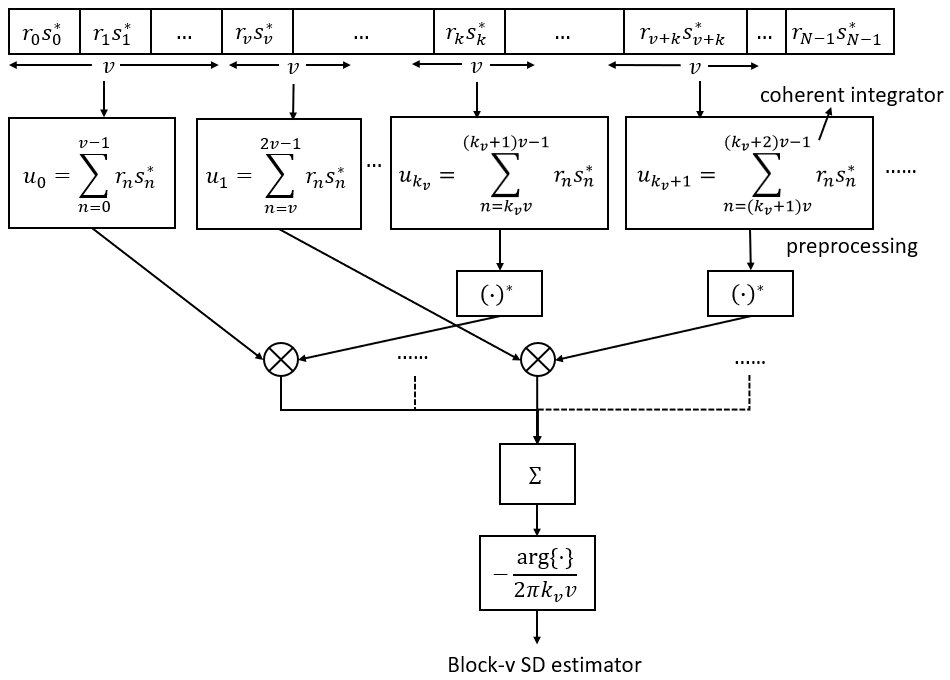
\includegraphics[width=3.4in,height=3.2in]{general_SD_estimator.png}}
  \caption{Flow diagram of implementing the Block-$v$ SD estimator}
  \label{fig:general_SD_estimator}
  \end{figure}

The reason for the primary SD e-stimator of~\eqref{eq:delta_SD} has a relatively bad performance at low SNR is because the large noise
disturbance significantly decorrelates the received signal and the preamble at each sample instant.
An alternative SD estimator is proposed by changing the order of computation in~\eqref{eq:delta_SD}.
Specifically, 
instead of calculating the correlation at each sample instant, 
cross-correlation between $k$ sample instant and then averaging, 
we first average the correlations for some coherent time instants; 
By doing this, some of processing gain is applied to increase the estimating accuracy in every small section of sample instants.
The results are called coherent integrators and the process is called preprocessing.
After that, use the remaining processing gain to integrate 
the coherent integrators between non-coherent time instants.
The details are illustrated in Figure~\ref{fig:general_SD_estimator}. 

In Figure~\ref{fig:general_SD_estimator}, the coherent integrator $u_l$ is formulated by

\begin{equation}
  \label{eq:coherent_integrator}
  u_l=\sum_{n=lv}^{(l+1)v-1}r_ns_n^*, \quad \text{for}~l=0,1,\ldots,N/v{-}1
\end{equation}
where $v$ denotes the number of coherent correlations that are for averaging. 
The value of $v$ is set to be a factor of $N$ to include all sample instants.
$k_v$ denotes the distance between coherent integrators 
that calculates correlation of non-coherent time instants.
Thus, $k_v=\lfloor k/v \rfloor$, where $\lfloor \cdot \rfloor$ represents the floor operation, since $v$ is not necessary to be a factor of $k$.
However, we still assume $k\approx k_vv$ for comparison simplicity. Based on above discussion, the alternative Block-$v$ SD estimator is given by

\begin{equation}
  \label{eq:general_sd_estimator}
  \hat{\delta}_{\text{Block}-v-\text{SD}}(v,k_v)=-\frac{\arg\big\{\sum_{l=k_v}^{N/v-1}u_l^*u_{l-k_v}\big\}}{2\pi k_vv}
\end{equation}
It can be seen that the primary SD estimator in~\eqref{eq:delta_SD} is a special case of Block-$v$ SD estimator when $v=1$.
Thus, we uniformly call the two estimators as the Block-$v$ SD estimator.

Now, we discuss the performance of Block-$v$ SD estimator by focusing on the cross-correlation between the two general coherent integrators in~\eqref{eq:general_sd_estimator}.
Based on~\eqref{eq:coherent_integrator} and the derivation of~\eqref{eq:ori_pdf_W}, the coherent integrator $u_l^*$ is complex Gaussian distributed with probability density function,

\begin{equation*}
  \label{eq:pdf_co_integrator_1}
  u_l^* \sim \cn\bigg(\frac{E_s/MS^*}{A^2}\sum_{n=lv}^{(l+1)v-1}e^{-j2\pi \bar{\delta}n},v\frac{E_s/M}{A^2}\frac{N_0}{2}\bigg),
\end{equation*}
and the pdf of complex Gaussian-distributed $u_{l-k_v}$ is also given by

\begin{equation*}
  \label{eq:pdf_co_integrator_2}
  u_{l-k_v} \sim \cn\bigg(\frac{E_s/MS}{A^2}\sum_{n=(l-k_v)v}^{(l-k_v+1)v-1}e^{j2\pi \bar{\delta}n},v\frac{E_s/M}{A^2}\frac{N_0}{2}\bigg).
\end{equation*}
Note, $u_l^*$ and $u_{l-k}$ are uncorrelated. Compared with~\eqref{eq:delta_extens_w_noise}, the cross-correlation between two coherent integrates $u_l^*$ and $u_{l-k_v}$ also yields a random variable
with a combination of Gaussian and second kind Bessel function. After some algebra, the mean and variance of $u_l^*u_{l-k_v}$, denoted as $\mu_{C_u}$ and $\sigma^2_{C_u}$, can be simplified by, respectively,

\begin{equation}
  \begin{aligned}
  \label{eq:cross_corr_co_inte}
  \mu_{C_u}&=\frac{(E_s/M)^2}{A^2}\sum_{n=lv}^{(l+1)v-1}e^{-j2\pi \bar{\delta}n}\Bigg(\sum_{m=(l-k)v}^{(l-k+1)v-1}e^{j2\pi \bar{\delta}m}\Bigg) \\
  &=\frac{(E_s/M)^2}{A^2}e^{-j2\pi \bar{\delta}k_vv}\Bigg(\frac{\sin(\pi \bar{\delta}v)}{\sin(\pi \bar{\delta})}\Bigg)^2, \\
  \sigma^2_{C_u}&=v^2\frac{(E_s/M)^2}{A^4}\Big(\frac{N_0}{2}\Big)^2+2v\frac{(E_s/M)^3}{A^4}\frac{N_0}{2}\Bigg(\frac{\sin(\pi \bar{\delta}v)}{\sin(\pi \bar{\delta})}\Bigg)^2,
\end{aligned}
\end{equation}
where $\frac{\sin(\pi \bar{\delta}v)}{\sin(\pi \bar{\delta})}$ is one of the Dirichlet function, which appro-aches the maximum value $v$ at $\bar{\delta}=0$ and the first pair of zero crossings at
$\bar{\delta}=\pm 1/v$. Based on~\eqref{eq:SNR_out_primary} and~\eqref{eq:cross_corr_co_inte}, 
the output SNR of Block-$v$ SD estimator in terms of the input SNR yields

\begin{equation}
  \begin{aligned}
    \label{eq:SNR_out_general}
    &\text{SNR}_{\text{out\_Block}-v}=\frac{|\mu_{C_u}|^2}{\sigma^2_{C_u}} \\
    &~~~=\frac{\frac{(Es/M)^4}{A^4}\Big(\frac{\sin(\pi \bar{\delta}v)}{\sin(\pi \bar{\delta})}\Big)^4(N/v-k_v)^2}
    {\Big[v^2\frac{(E_s/M)^2}{A^4}\Big(\frac{N_0}{2}\Big)^2+2v\frac{(E_s/M)^3}{A^4}\frac{N_0}{2}\Big(\frac{\sin(\pi \bar{\delta}v)}{\sin(\pi \bar{\delta})}\Big)^2\Big](N/v{-}k_v)} \\
    &~~~=\frac{(N/v-k_v)\Big(\frac{\sin(\pi \bar{\delta}v)}{\sin(\pi \bar{\delta})}\Big)^4}
    {\frac{v^2}{\text{SNR}_{\text{in}}^2}+\frac{2v}{\text{SNR}_{\text{in}}}\Big(\frac{\sin(\pi \bar{\delta}v)}{\sin(\pi \bar{\delta})}\Big)^2}.
  \end{aligned}
\end{equation}
Some important observations of $\text{SNR}_{\text{out\_Block}-v}$ from~\eqref{eq:SNR_out_general} can be discussed. 
  First, the $\text{SNR}_{\text{out}}$ depends on the value of $|\bar{\delta}|v$.
We begin to consider the case when $|\bar{\delta}|v\ll1$, i.e., $\frac{\sin(\pi \bar{\delta}v)}{\sin(\pi \bar{\delta})} \approx v$
and $(N/v-k_v)v \approx N-k$.
When the input SNR is moderate, the second term of variance dominates and results the nearly same output SNR as in~\eqref{eq:SNR_out_primary};
While at low SNR, the first term of variance dominates and ideally produces an approximate $v$ times larger output SNR than the primary SD estimator,
whi-ch corresponds to the design intention of block-$v$ ($v \geq 2$) SD estimator.
The selection of $v$ trades off the processing gain at low SNR and incurred large frequency offset.

In practice, $|\bar{\delta}|$ is generally not large,
a reasonable assump-tion is to assume $\bar{\delta}$ is in the range of $[-1/v,1/v]$.
By com-paring~\eqref{eq:SNR_out_primary} and~\eqref{eq:SNR_out_general}, it is easy to get
the Block-$v$ SD estimator produces a positive processing gain at low SNR when $|\bar{\delta}|v$ satisfies
$\frac{\sin(\pi \bar{\delta}v)}{\sin(\pi \bar{\delta})} \in [v^{3/4},v]$;
However, The worst case happens when $|\bar{\delta}|v_{\text{min}}$ even also produces a relative large frequency offset, 
i.e., $v_{\text{min}}=2$ and $\frac{\sin(2\pi \bar{\delta})}{\sin(\pi \bar{\delta})}\in [0,2^{3/4})$; 
The Block-$v$ SD estimator will not improve the performance than the primary SD estimator at low SNRs.

Now, let's measure the distribution of Block-$v$ SD estimator at low SNR.
Assume $|\bar{\delta}|v$ always satisfies $v^{3/4}\leq\frac{\sin(\pi \bar{\delta}v)}{\sin(\pi \bar{\delta})}\leq v$,
and the extra processing gain $v$ at relatively low SNR increases the $\text{SNR}_{\text{out\_Blv}}$ to meet the moderate SNR requirement of~\eqref{eq:sol_pdf_W}.
Thus, by plugging~\eqref{eq:cross_corr_co_inte},~\eqref{eq:sol_pdf_W} into~\eqref{eq:general_sd_estimator}, the block-$v$ SD estimator is distributed approximately Gaussian at relatively low SNR with probability density function

\begin{equation}
  \begin{aligned}
  \label{eq:pdf_general_delta}
      \est{\delta}{\text{Block}-v-\text{SD}}(&v,k_v) \\
      &\sim \n \bigg(\bar{\delta},\frac{M^2v^2}{16\pi^2k^2\Big(\frac{\sin(\pi \bar{\delta}v)}{\sin(\pi \bar{\delta})}\Big)^4(N/v{-}k_v)(E_s/N_0)^2}\bigg).
  \end{aligned}
\end{equation} 
Thus, $\est{\delta}{\text{Block}-v-\text{SD}}$ is also unbiased. Moreover, the lag $k_v$ also affects the variance of Block-$v$ SD estimator. The best choice is to choose
$k_v=\lfloor\frac{2N}{3v}\rfloor$ to minimize the variance. However,
it should be noted that if $k_vv$ is too large, 
the frequency estimate $\est{\delta}{\text{Block}-v-\text{SD}}$ 
may suffer the effect of "alasing" if $2\pi|\bar{\delta}|k_vv>\pi$.
The ambiguity problems are common in frequency estimation. The effective method to solve it is based on the robust Chinese reminder theorem.
% should give some reference.

It should be also compared and emphasized the complexity of block-$v$ ($v\geq 2$) SD estimator
with block-1 SD estimator in sequential detection process. The two estimators have the same
complexity for single detection but large computational-complexity difference in sequential detection.
Note, for block-$v$ ($v\geq 2$) SD estimator, because of preprocessing, each sample in received sequence should
be multiplied by the sample in the preamble at same sample instant; 
This greatly limits the way of computing between two adjacent sequential detection.
However, for block-1 SD estimator in~\eqref{eq:delta_SD}, the more efficient way is to 
calculate the autocorrelations for both received and reference sequence with sample difference $k$ and then multiply.
By doing this method, except for the first received sequence,     
we only need to calculate one more autocorrelation for the incoming sample at each detection.
Since the autocorrelations of samples in the preamble can be pre-computed, the argument of~\eqref{eq:delta_SD}
can be computed by the cross-correlation between 
the autocorrelations of received sequence in a shift register
and autocorrelations of reference samples in a fixed vector. 
Thus, compared with block-$v$, block-1 SD estimator greatly reduces the computational redundancy in sequential detection.

\subsection{Solution II: (Fine) Newton-Method (NM) Estimator}

The (block-$v$) SD estimator emphasizes the low-complexity property and is intended to provide merely sufficiently good carrier synchronization
to enable coherent detection. 
Once the signal has been acquired, the accuracy of the block-$v$ SD estimator can be improved by 
investing additional computations. Since detection events are rare, the computational complexity is of little concern.

The principle is to use the Block-$v$ SD estimator as the starting point for a Newton-type iteration 
aimed at finding a better solution to the necessary condition~\eqref{eq:delta}. 
In principle, multiple iterations are possible to produce successively better approximations to the root of
$\J(\hat{\delta})$ in~\eqref{eq:delta}. Specifically, the iterations are given by

\begin{equation}
    \label{eq:iter_NM_est}
    \est{\delta}{\nm}^{(i+1)}=\est{\delta}{\nm}^{(i)}-
    \frac{\J(\est{\delta}{\nm}^{(i)})}{\J^\prime(\est{\delta}{\nm}^{(i)})}
  \end{equation}
where $\est{\delta}{\nm}^{(0)}~{=}~\est{\delta}{\sd}(k_{\opt})$ is the starting point of the iteration and
$\J^\prime(\cdot)$ denotes the derivative of $\J$ with respect to $\hat{\delta}$. Specifically,

\begin{equation}
    \label{eq:derivative of delta}
    J^\prime(\hat{\delta}) = \Im\bigg\{\sum_{k=1}^{N-1}{\sum_{m=k}^{N-1}{j2\pi k^2r_{m-k}r_m^{*}s_{m-k}^{*}s_m}e^{j2\pi\hat{\delta}k}}\bigg\}.
    \end{equation}
Our simulations indicate that only a single iteration is usually sufficient to achieve very good accuracy.




\section{Simulation Results}%
\label{sec:simulations}

\begin{figure}[t]
    \centerline{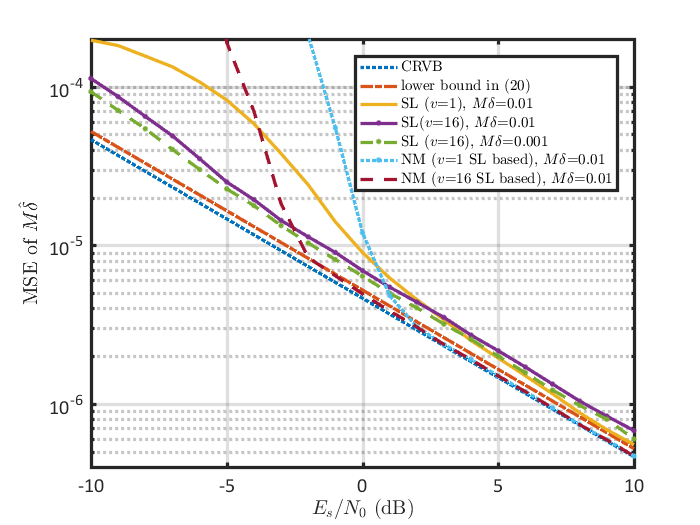
\includegraphics[width=3.15in]{accuracy_NM_SL.png}}
    \caption{Accuracy of the NM and the SL estimators ($L_0=32$, $M=2$)}
    \label{fig:accuracy_NM_SL}
    \end{figure}

In the simulation section, we reverse the order of discussion by first showing 
the accuracy of estimators in carrier synchronization and then showing some results of sequential detection since
the GLRT based detector in~\eqref{eq:generalized_corr} relies on the accuracy of 
the SL estimator.
The symbol sequence of the preamble is chosen as a Gold sequence 
with good autocorrelation properties and
modulated by a QPSK alphabet.
The pulse is chosen as a
Square-Root Raised Cosine (SRRC) pulse with roll-off equal to 0.5.
The normalized frequency offset $\delta$ is intentionally set to be in
the safe estimation range for all estimators for simulation purposes. 

\subsection{Simulation Results for Estimation}%

% \begin{figure}[t]
%     \centerline{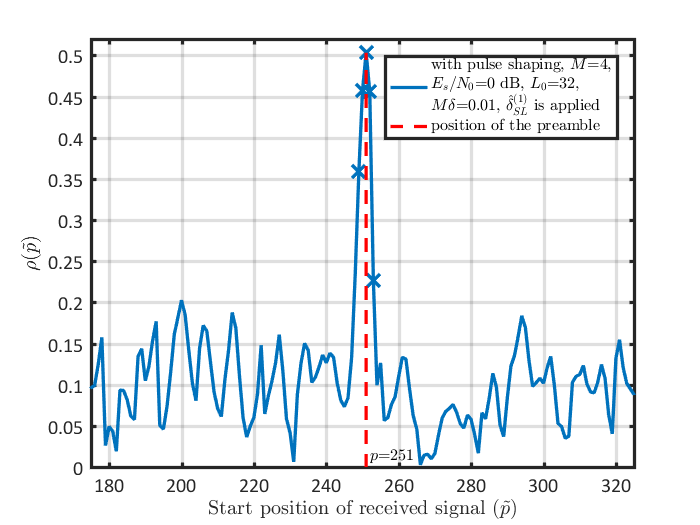
\includegraphics[width=3.4in]{generalized_correlation_p_plus_delta.png}}
%     \caption{Performance of sequential detector when the preamble is pulse shaped}
%     \label{fig:Generalized correlation}
%     \end{figure}

Fig.~\ref{fig:accuracy_NM_SL} illustrates the accuracy of the single-lag (SL) estimator and the NM estimator.
Comparing the two curves for the SL estimators with $v=1$ and $v=32$, 
we see the length-$32$ partial integration
improves the accuracy by providing an approximate
\SI{4}{\dB}~performance gain at negative SNRs
(near $\text{SNR}=\SI{-5}{\dB}$). This is consistent
with~\eqref{eq:relative_processing_gain}.

The SL estimator with $v=1$ is slightly more accurate
at \SI{10}{\dB}~SNR than the one with $v=32$.
The gap is due to the Dirichlet function.
% for $\delta \neq 0$.
%For the same reason,
Also, when $v>1$
the accuracy of the estimator improves at all SNRs as $|\delta|$ decreases.
% When  $\delta$ is very small, the accuracy of the SL estimator with $v=32$ has better accuracy at all SNRs.

The SL estimators do not approach the Cramer-Rao Vector Bound (CRVB)~\cite{Gini_98} while the NM
estimators do at moderate SNR. 
% We also see that the
The NM estimator achieves improved accuracy at lower SNR
when the SL estimator with $v=32$ is used as the starting point. 
In contrast, at all negative SNRs the NM estimator based on SL estimation with $v=1$ has
worse accuracy than SL estimation alone.
This is because the accuracy of the SL estimator is not sufficient to
provide a consistently good starting point and the Newton iteration converges occasionally to 
other local minima away from the true frequency offset.

Fig.~\ref{fig:accuracy_NM_SL_traditional} compares the accuracy of our  estimators
and the (more complex) estimators in~\cite{kay_89,Fitz_94,Luise_Reggiannini_95}.
For small
frequency offset, the NM estimator has a slightly better accuracy than other estimators at moderate SNRs.
In general, our family of  SL estimators with different block lengths $v$
are very competitive across all SNRs considered here while maintaining
low computational complexity that allows for real-time application.

\begin{figure}[t]
    \centerline{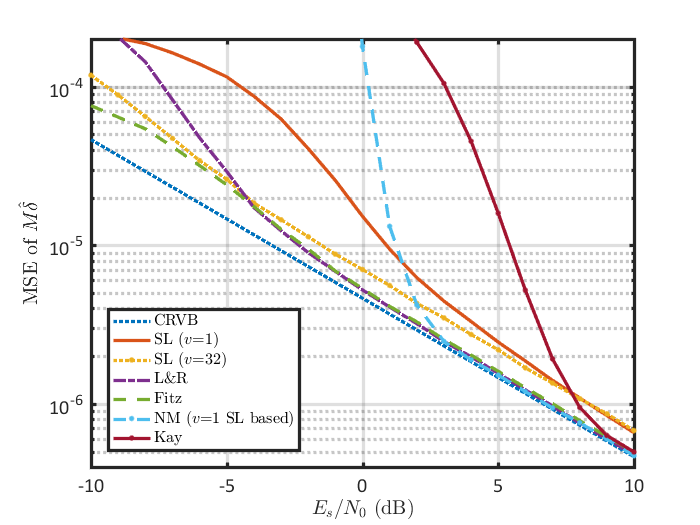
\includegraphics[width=3.15in]{accuracy_NM_SL_traditional.png}}
    \caption{Accuracy of the SL, the NM and the traditional estimators ($L_0=32$, $M=2$, $M\delta=0.01$)}
    \label{fig:accuracy_NM_SL_traditional}
    \end{figure}

\begin{figure}[t]
  \centerline{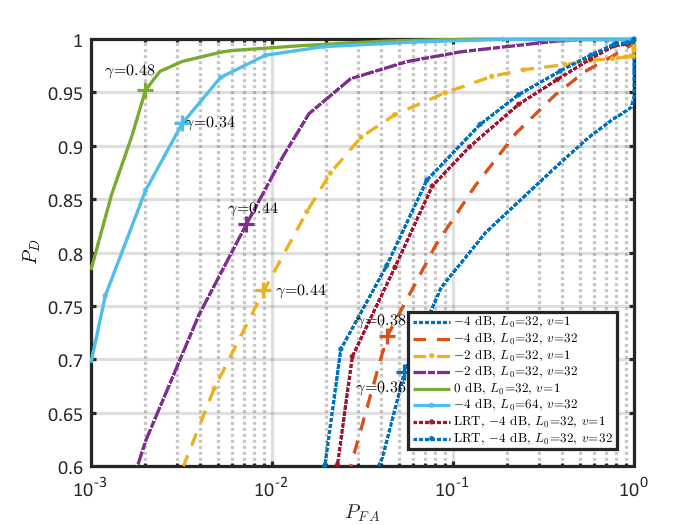
\includegraphics[width=3.15in]{ROC_new.png}}
  \caption{Receiver operating characteristics (ROC) of the sequential detector ($M=2$, $M\delta=0.01$)}
  \label{fig:Receiver operating characteristics}
\end{figure}


\subsection{Simulation Results for Detection}

% Figure~\ref{fig:Generalized correlation} shows the performance of sequential detector
% in~\eqref{eq:generalized_corr} at each received signal windows. Note, because of pulse sha-ping,
% the autocorrelation property of the preamble sequence is decreased, which results
% the correlations at adjacent windows near the position of the preamble decay slow and thus make much challenges
% to choose threshold to make correct dicision.

% The solution is to adjust the detection algorithm by finding the local maximum of the correlation
% instead of just comparing the correlation with the threshold at each window. Note, when count for the ratio of false alarm and detection (for determining the threshold),
% the two positions should be counted as latter.


Fig.~\ref{fig:Receiver operating characteristics} shows the receiver
operating characteristics (ROC) of the detection algorithm. 
The better accuracy of SL estimation with partial integration also
improves the detection performance  at low SNR.
For example, at $\SI{-2}{\dB}$ SNR, $\gamma=0.44$, the false alarm probability $P_{FA}$ of SL with $v=32$ is reduced $0.2\%$ and 
the detection probability $P_{D}$ is $5\%$ larger compared with the SL with $v{=}1$. 
Fig.~\ref{fig:Receiver operating characteristics} also shows the detector does not work well at $\SI{-4}{\dB}$ SNR if only $32$ symbols of preamble are used;  
The performance is significantly improved by doubling the length of
the preamble. The two curves marked LRT at $\SI{-4}{\dB}$ SNR with different $v$
are obtained by plugging in the true frequency and phase offsets as an upper bound for comparing with 
the results of the GLRT.   

% \begin{figure}[t]
%   \centerline{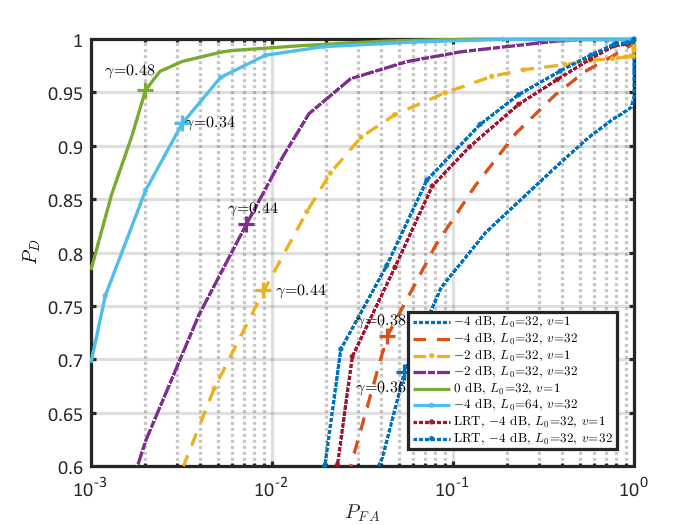
\includegraphics[width=3.15in]{ROC_new.png}}
%   \caption{Receiver operating characteristics (ROC) of the sequential detector ($M=2$, $M\delta=0.01$)}
%   \label{fig:Receiver operating characteristics}
% \end{figure}



\section{Implementation on Software-defined radio}
\label{sec:real_implementation}

\begin{figure*}[t]
  \centerline{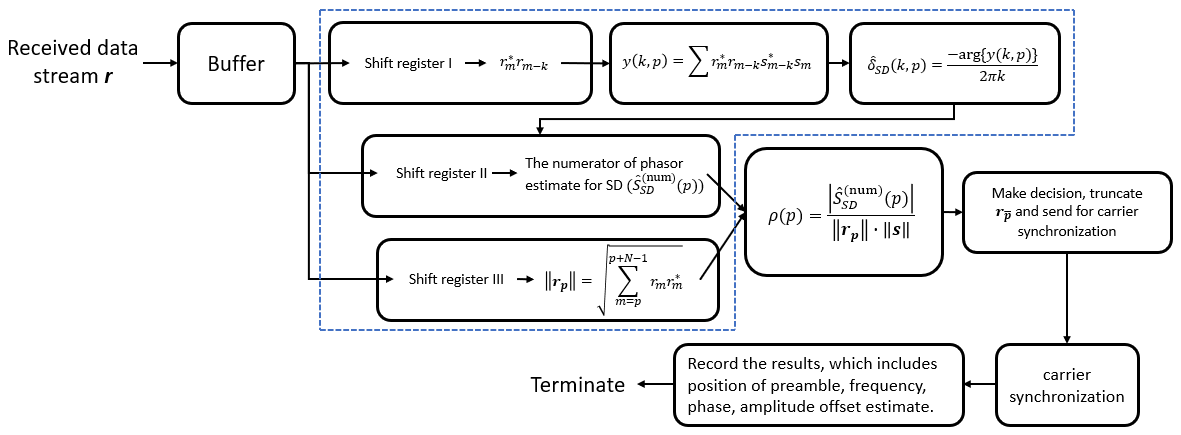
\includegraphics[width=6.5in]{SDR_receiver.png}}
  \caption{Block diagram for implementing the proposed algorithm on software-defined radio (some steps are omitted)}
  \label{fig:SDR_receiver}
  \end{figure*}

Two main aspects of measuring the performance of modern communcation systems, except for accuracy,
are the latency and throughput. In the previous sections, we focus on explaining and showing
how much accuracy of our proposed joint detection and estimation algorithm can be.
In order to realize it on software-defined radio (SDR), the algorithm, especially the detection algorithm, should be refined
to fitting very high sample rate since it is applied on every time instant.

\subsection{Receiver Side (algorithm)}

Figure~\ref{fig:SDR_receiver} illustrates some detailed changes of our proposed algorithm.
First, the style of the observation window with feedback loop in Figure~\ref{fig:sig_acquis_chain} is eliminated
because it incurs a very large amount of overhead. Instead, the received data is directly buffered into 
a fixed size (normally larger than the length of the preamble) of frame without overlapping. Now
the problem may happen when the preamble in the received data is cut off over two frames. 
The shift register is reused after the buffer to solve this problem. Compared with the old method, the received data packed in frames can be processed in order without
waiting for the result of detecting; Moreover, the length of the shift register can be also reduced. 
For example, if we look at formula of the SD estimator in~\eqref{eq:delta_SD}, the length of the shift register can be shortened from $N$ to $k+1$,
i.e., if $k=\frac{2}{3}N$, the overhead is approximately reduced by $\frac{N}{3}$.

Second, some key steps of the proposed detection algorithm should be computed more efficiently.
For example, to calculate the frequency estimate of SD estimator,~\eqref{eq:delta_SD} can be intepreted as the convolution between autocorrelation vector of received samples and of the preamble (one of them should be reversed). 
Thus, the most efficient way of calculating~\eqref{eq:delta_SD} could be the fast fourier transform (FFT). 

Another important improvement that should be emphasized is about calculating the phase (phasor) estimate
of the SD estimator in~\eqref{eq:opt_S}. No
te,~\eqref{eq:opt_S} is a time-varying convolution, which cannot be computed by FFT.
To approximate the dot product in~\eqref{eq:opt_S}, we re-order the computation by first calculating the dot product between the (partial) received data vector ($\bm{r}$) and the (partial) preamble ($\bm{s}$);
the result is then corrected (multiplied) by the frequency estimate at the middle position of data vector and added together. Specifically, the numerator of

\begin{equation}
    \label{eq:refined_opt_S}
    \hat{S} \approx \sum_{i=0}^{L_2-1} \sum_{m=iL_1/L_2}^{(i+1)L_1/L_2-1}
    \sum_{n=mN/L_1}^{(m+1)N/L_1-1}r_ns_n^* 
    e^{-j\pi \hat{\delta}\frac{N(2m+1)}{L_1}}.
  \end{equation}
As illustrated in Figure~\ref{fig:SDR_receiver}, we compute~\eqref{eq:refined_opt_S} in two stages, each
stage contains $L_1$ (or $L_2$) parallel sub cells. 
Thus, we achieve the functional parallelism by an approximate of $L_1 \cdot L_2$ speed up.
To get a good approximation, $L_1$ should not be too small and 
$L_2$ is the factor of $L_1$.

\subsection{Signal Transmission Path}

In this section, we briefly talk about the signal transmitting path, which is used 
for testing our algorithm. The hardware connection is fairly easy. 
Each of two processors (computers) connected to a universal software radio peripheral (USRP) 
by one 5-Gigabit Ethernet cable as the transmitter or receiver. Between two USRPs,
a cable with~\numb{30}\dB~attenuation connects the RX/TX port and RX port.
At the transmitter side, the processor needs to tell the (transmitter) USRP the sample rate, 
the baseband signal and frequency, the carrier frequency, the transmitter gain, etc. 
Then, the USRP transmits the analog signal to the (receiver) USRP through the two ports.
At the receiver side, the received analog RF signal is first down-converted to baseband, down-sampled to 
discrete-time data stream and finally stored in the local network. After that, our proposed algorithm as illustrated
in Figure~\ref{fig:SDR_receiver} can be tested by requesting the data from the local network.

\subsection{Performance of SDR}

To measure the performance of the SDR, we focus on the accuracy, throughput and latency of our proposed algorithm.
Some parameters in Figure~\ref{fig:SDR_receiver} should be chosen by the following rules:
First, the length of the preamble should be chosen short enough to get the largest throughput as long as it does not degrade the accuracy;
Second, the length of frame should be chosen as the power of 2 to achieve the best performance of FFT; Moreover, 
it trades off between the overhead and latency, e.g., short frame has small latency but large overhead. 
Third, as discussed above, $L_1$ in~\eqref{eq:refined_opt_S} should not be chosen too small for a good approximation of phasor estimate. However, the large number of 
parallel executions will occupy the most threads of the computer.

As tested, such parameters are determined that can achieve a relatively good performance: 
The preamble is chosen with the number of symbols $L_0=32$ and oversampling factor $M=4$.
the length of the frame is determined by 8192; Four complete preambles are embedded in each frame. 
The number of sub cells for two stages are $L_1=2L_2=16$. Furthermore, some parameters of USRP are set as follows:
The sample rate at transmitter is 10 MS/s; The transmitter gain plus receiver gain is~\numb{20}\dB.
Based on above, we get the maximum throughput is around 4.5 MS/s and the latency is near 1 ms;
The detection algorithm is very robust and the false alarm probability is near 0.




% % extension to reviewer 1, comment 8
% \input{conclusion} can be finished later

% extension to reviewer 1, comment 6, reviewer 3, comment 4
\begin{appendices}

\section{Derivation of distribution for the SD estimator, proof of (\ref{eq:sol_pdf_W})}
\label{AL}

To prove the distribution of $\arg\{W(k)\}$, where $W(k)$ is a complex Gaussian 
random variable, we assume $W=X+jY$, $X$ and $Y$ are two Gaussian random 
variables with distributions $X {\sim} \n(\mu_x,\sigma^2)$ 
and $Y {\sim} \n(\mu_y,\sigma^2)$. Here, $W$, $X$, $Y$, $\mu_x$, $\mu_y$ 
and $\sigma^2$ all depends on $k$, we just write those for notation simplicity. 
We further assume $\mu_w$ to be the mean of $W$. The probability density function 
of $W$ is given by

\begin{equation}
    \label{eq:AL1}
    \begin{aligned}
    &f_W(w) \\
    &{=}f_{X,Y}(x,y){=}\frac{1}{2\pi \sigma^2}\exp\bigg({-}\frac{(x-\mu_x)^2+(y-\mu_y)^2}{2\sigma^2}\bigg).
    \end{aligned}
\end{equation}
Let $x=r\cos\theta$, $y=r\sin\theta$,~\eqref{eq:AL1} can be transformed into polar coordinate,

\begin{equation}
    \label{eq:AL2}
    \begin{aligned}
    &f_W(w){=} f_{R,\Theta}(r,\theta) \\
    &{=}\frac{r}{2\pi \sigma^2}\exp\bigg({-}\frac{(r\cos\theta-\mu_x)^2+(r\sin\theta-\mu_y)^2}{2\sigma^2}\bigg) \\
    &{=}\frac{r}{2\pi \sigma^2}\exp\bigg({-}\frac{r^2{+}\mu_x^2{+}\mu_y^2}{2\sigma^2}\bigg)\exp\bigg(\frac{r}{\sigma^2}(\mu_x\cos\theta{+}\mu_y\sin\theta)\bigg)
    \end{aligned}
\end{equation}
Plugging $\mu_x=|\mu_w|\cos(\angle\mu_w)$, $\mu_y=|\mu_w|\sin(\angle\mu_w)$ yields

\begin{equation}
    \label{eq:AL3}
    \begin{aligned}
    &f_{R,\Theta}(r,\theta) \\
    &{=}\frac{r}{2\pi \sigma^2}\exp\bigg({-}\frac{r^2+|\mu_w|^2}{2\sigma^2}\bigg)\exp\bigg(\frac{r|\mu_w|}{\sigma^2}\cos(\theta{-}\angle\mu_w)\bigg).
    \end{aligned}
\end{equation}
Note that $\theta=\arg\{W(k)\}$. Thus, we turn our attention to mar\-ginal PDF of $\theta$, 

\begin{equation}
    \label{eq:AL4}
    \begin{aligned}
    &f_\Theta(\theta) {=}\int_{0}^{\infty}\frac{r}{2\pi  \sigma^2}\exp\bigg({-}\frac{r^2{-}2r|\mu_w|\cos(\theta{-}\angle\mu_w){+}|\mu_w|^2}{2\sigma^2}\bigg)dr \\
    &{=}\int_{0}^{\infty}\frac{r}{2\pi\sigma^2} \cdot\\
    &\exp\bigg({-}\frac{(r{-}|\mu_w|\cos(\theta{-}\angle{\mu_w}))^2{+}|\mu_w|^2(1{-}\cos^2(\theta{-}\angle\mu_w))}{2\sigma^2}\bigg)dr \\
    &{=}\frac{1}{2\pi}\exp\bigg({-}\frac{|\mu_w|^2(1{-}\cos^2(\theta-\angle\mu_w))}{2\sigma^2}\bigg) \cdot \\
    &\int_{0}^{\infty}\frac{r}{\sigma^2}\exp\bigg({-}\frac{(r{-}|\mu_w|\cos(\theta{-}\angle{\mu_w}))^2}{2\sigma^
    2}\bigg)dr.
    \end{aligned}
\end{equation}
By assuming

\begin{equation*}
\begin{aligned}
    &\alpha{=}|\mu_w|\sin(\theta{-}\angle\mu_w) \\
    &\beta{=}|\mu_w|\cos(\theta{-}\angle\mu_w) \\
    &u{=}\frac{r{-}|\mu_w|\cos(\theta{-}\angle\mu_w)}{\sigma},
    \end{aligned}
\end{equation*}
\eqref{eq:AL4} can be simplified as

\begin{equation}
    \label{eq:AL5}
    \begin{aligned}
    f_\Theta(\theta) &{=}\frac{1}{2\pi}\exp\bigg({-}\frac{\alpha^2}{2\sigma^2}\bigg)\int_{{-}\frac{\beta}{\alpha}}^{\infty}\bigg(u{+}\frac{\beta}{\alpha}\bigg)\exp\bigg({-}\frac{u^2}{2}\bigg)du \\
    &{=}\frac{1}{2\pi}\exp\bigg({-}\frac{\alpha^2}{2\sigma^2}\bigg)\bigg(\int_{{-}\frac{\beta}{\alpha}}^{\infty}ue^{{-}\frac{u^2}{2}}du+\int_{{-}\frac{\beta}{\alpha}}^{\infty}\frac{\beta}{\alpha}e^{{-}\frac{u^2}{2}}du\bigg) \\
    &{=}\frac{1}{2\pi}\exp\bigg({-}\frac{\alpha^2{+}\beta^2}{2\sigma^2}\bigg){+}\frac{\beta}{\sqrt{2\pi}\sigma}\exp\bigg({-}\frac{\alpha^2}{2\sigma^2}\bigg)\Q\bigg({-}\frac{\beta}{\alpha}\bigg) \\
    &{=}\frac{1}{2\pi}\exp\bigg({-}\frac{|\mu_w|^2}{2\sigma^2}\bigg){+}\frac{|\mu_w|\cos(\theta{-}\angle\mu_w)}{\sqrt{2\pi}\sigma} \cdot \\
    &\exp\bigg({-}\frac{|\mu_w|^2\sin^2(\theta{-}\angle\mu_w)}{2\sigma^2}\bigg)\Q\bigg({-}\frac{|\mu_w|}{\sigma}\cos(\theta{-}\angle\mu_w)\bigg)
    \end{aligned}
\end{equation}
where $\Q(\cdot)$ is the $\Q$ function and~\eqref{eq:AL5} gives the explicit 
mar\-ginal PDF for $\theta$. Note that $|\mu_w|=(N-k)(\frac{E_s}{T})^2$ 
from~\eqref{eq:ori_pdf_W}. Thus, at relatively high SNR, i.e., $|\mu_w|\gg\sigma$,
~\eqref{eq:AL5} can be approximated by

\begin{equation}
    \label{eq:AL6}
    \begin{aligned} 
    &f_\Theta(\theta) \approx \frac{1}{2\pi}\exp\bigg({-}\frac{|\mu_w|^2}{2\sigma^2}\bigg)\\
    &+\frac{|\mu_w|\cos(\theta{-}\angle\mu_w)}{\sqrt{2\pi}\sigma} 
    \exp\bigg({-}\frac{|\mu_w|^2\sin^2(\theta{-}\angle\mu_w)}{2\sigma^2}\bigg) \cdot \\
    &\bigg(1{-}\frac{\sigma}{\sqrt{2\pi}|\mu_w|\cos(\theta{-}\angle\mu_w)}\exp\bigg({-}\frac{|\mu_w|^2\cos^2(\theta{-}\angle\mu_w)}{2\sigma^2}\bigg)\bigg) \\
    &=\frac{|\mu_w|\cos(\theta{-}\angle\mu_w)}{\sqrt{2\pi}\sigma}\exp\bigg({-}\frac{|\mu_w|^2\sin^2(\theta{-}\angle\mu_w)}{2\sigma^2}\bigg)
    \end{aligned}
\end{equation}
The approximation holds because of the property of $\Q$ function 
$Q(x) \approx\frac{1}{\sqrt{2\pi x}}\exp\big({-}\frac{x^2}{2}\big)$ 
for $x\gg 0$. Then, we only need to look at $f_\Theta(\theta)$ where 
$\theta \approx \angle\mu_w$, i.e.,

\begin{equation}
    \label{eq:AL7}
    f_\Theta(\theta) \approx \frac{|\mu_w|}{\sqrt{2\pi}\sigma}\exp\bigg({-}\frac{|\mu_w|^2}{2\sigma^2}(\theta{-}\angle\mu_w)^2\bigg)
\end{equation}
Thus, $\theta$ is approximately Gaussian with the distribution 
$\theta \sim \n \big(\angle \mu_{W},\frac{\sigma^2}{|\mu_{W}|^2}\big)$, 
which is equivalent to~\eqref{eq:sol_pdf_W}.

\section{Derivation of the CRVB for frequency and phase estimate, 
proof of~\eqref{eq:CRVB_freql} and~\eqref{eq:CRVB_phi}}

\label{BL}

In order to derive the CRVB for joint estimation of phase and frequency 
offset, We define a parameter vector $\bm{\theta}{\triangleq}\begin{bmatrix} \delta&\phi \end{bmatrix}$ 
to include the two parameters that we want to estimate. 
The first step towards the derivation of the CRVB is to compute 
the Fisher Information Matrix (FIM, $\bm{I}(\bm{\theta})$). 
The calculation of $\bm{I}(\bm{\theta})$ is based on log-likelihood 
function ($\ln\Lambda$), which is carried out in \cite[Ch.~4]{VanTrees_vol1}

\begin{equation}
\label{eq:log_likelihood_func}
\ln\Lambda[r(t),\bm{\theta}]{=}\frac{2}{N_{0}}\int_{0}^{T_{0}}r(t)s'^{*}(t,\bm{\theta})dt{-}\frac{1}{N_{0}}\int_{0}^{T_{0}}|s'(t,\bm{\theta})|^{2}dt
\end{equation}
where 

\begin{equation}
\label{eq:log_lik_func_comp}
s'(t,\bm{\theta})=Ae^{j(2\pi\delta t+\phi)}\sum_{i=0}^{L_{0}-1}c_{i}g(t-iT),
\end{equation}
and $T_{0}$ is the observation length. Taking the second derivative with respect to each element of the parameter vector $\theta_{i}$, $\theta_{j}$ yields

\begin{equation}
\begin{aligned}
\label{eq:double_derivative_theta}
&\frac{\partial^2\ln\Lambda}{\partial\theta_{i}\partial\theta_{j}} \\
&{=}\frac{2}{N_{0}}\int_{0}^{T_{0}}r(t)\frac{\partial^2 s'^{*}(t,\bm{\theta})}{\partial \theta_{i}\partial \theta_{j}}dt
-\frac{2}{N_{0}}\int_{0}^{T_{0}}\frac{\partial s'^{*}(t,\bm{\theta})}{\partial \theta_{i}}\frac{\partial s'(t,\bm{\theta})}{\partial \theta_{j}}dt \\
&-\frac{2}{N_{0}}\int_{0}^{T_{0}}s'(t,\bm{\theta})\frac{\partial^2 s'^{*}(t,\bm{\theta})}{\partial \theta_{i}\partial \theta_{j}}dt.
\end{aligned}
\end{equation}
Taking the negative expectation of (\ref{eq:double_derivative_theta}), the elements of FIM are given by

\begin{equation}
\label{eq:FIM}
\bm{I}(\bm{\theta})_{ij}=-\E\left[\frac{\partial^2 \ln\Lambda}{\partial \theta_{i}\partial \theta_{j}}\right]=\frac{2}{N_{0}}\int_{0}^{T_{0}}\frac{\partial s'^{*}(t,\bm{\theta})}{\partial \theta_{i}}\frac{\partial s'(t,\bm{\theta})}{\partial \theta_{j}}dt.
\end{equation}
By plugging $s'(t,\bm{\theta})$ from (\ref{eq:log_lik_func_comp}) into (\ref{eq:FIM}) 
and replacing $\theta_{i}$, $\theta_{j}$ with $\delta,\delta$, 
the first element of FIM ($\bm{I}(\bm{\theta})_{11}$) yields

\begin{equation}
\label{eq:FIM_delta_delta}
\begin{aligned}
\bm{I}(\bm{\theta})_{11}&=\frac{2}{N_{0}}\int_{0}^{T_{0}}\frac{\partial Ae^{j(2\pi\delta t+\phi)}\sum_{i=0}^{L_{0}-1}c_{i}g(t{-}iT)}{\partial \delta} \cdot \\
&\frac{\partial Ae^{-j(2\pi\delta t+\phi)}\sum_{i=0}^{L_{0}-1}c_{i}^{*}g^{*}(t{-}iT)}{\partial \delta}dt \\
&=\frac{2}{N_{0}}\int_{0}^{T_{0}}A^{2}4\pi^{2}t^{2}\left|\sum_{i=0}^{L_{0}-1}c_{i}g(t{-}iT)\right|^{2}dt.
\end{aligned}
\end{equation}
Note that the averaged symbol energy of transmitted signal is calculated by
\begin{equation}
\label{eq:avg_symbol_energy}
\begin{aligned}
E_{s}&=\int_{0}^{T}\left|A\sum_{i=0}^{L_{0}-1}c_{i}g(t{-}iT)\right|^{2}dt \\
&\approx\sum_{k=0}^{M-1}\left|A\sum_{i=0}^{L_{0}-1}c_{i}g(kT_s-iT)\right|^{2}T_{s} \\
&\approx T\left|A\sum_{i=0}^{L_{0}-1}c_{i}g(t-iT)\right|^{2},
\end{aligned}
\end{equation}
or,

\begin{equation}
\label{eq:avg_symbol_energy_deriv}
A^{2}\left|\sum_{i=0}^{L_{0}-1}c_{i}g(t{-}iT)\right|^{2}{\approx}\frac{E_{s}}{T}.
\end{equation}
where $M=\text{int}(T/T_{s})$. The first approximation in~\eqref{eq:avg_symbol_energy} 
is based on Riemann sum theory. $\bm{I}(\bm{\theta})_{11}$ finally results in

\begin{equation}
\label{eq:FIM_delta_delta_result}
\bm{I}(\bm{\theta})_{11}=\frac{8\pi E_{s}T_{0}^2L_{0}}{3N_{0}}.
\end{equation}
Similarly, $\bm{I}(\bm{\theta})_{12}$ can be calculated by plugging $s'(t,\bm{\theta})$ from (\ref{eq:log_lik_func_comp}) into (\ref{eq:FIM}) and replacing $\theta_{i}$, $\theta_{j}$ with $\delta,\phi$, which is given by

\begin{equation}
\label{eq:FIM_delta_phi}
\begin{aligned}
\bm{I}(\bm{\theta})_{12}&=\frac{2}{N_{0}}\int_{0}^{T_{0}}\frac{\partial Ae^{j(2\pi\delta t+\phi)}\sum_{i=0}^{L_{0}-1}c_{i}g(t{-}iT)}{\partial \delta} \cdot \\
&\frac{\partial Ae^{-j(2\pi\delta t+\phi)}\sum_{i=0}^{L_{0}-1}c_{i}^{*}g^{*}(t{-}iT)}{\partial \phi}dt.
\end{aligned}
\end{equation}
Following the same steps as deriving $\bm{I}(\bm{\theta})_{11}$, $\bm{I}(\bm{\theta})_{12}$ can be finally reduced to
\begin{equation}
\label{eq:FIM_delta_phi_result}
\bm{I}(\bm{\theta})_{12}=\frac{2\pi E_{s}T_{0}L_{0}}{N_{0}}.
\end{equation}
$\bm{I}(\bm{\theta})_{22}$ can be calculated by plugging $s'(t,\bm{\theta})$ from (\ref{eq:log_lik_func_comp}) into (\ref{eq:FIM}) and replacing $\theta_{i}$, $\theta_{j}$ with $\phi,\phi$, which is given by

\begin{equation}
\label{eq:FIM_phi_phi}
\begin{aligned}
\bm{I}(\bm{\theta})_{22}&=\frac{2}{N_{0}}\int_{0}^{T_{0}}\frac{\partial Ae^{j(2\pi\delta t+\phi)}\sum_{i=0}^{L_{0}-1}c_{i}g(t{-}iT)}{\partial \phi} \cdot \\
&\frac{\partial Ae^{-j(2\pi\delta t+\phi)}\sum_{i=0}^{L_{0}-1}c_{i}^{*}g^{*}(t{-}iT)}{\partial \phi}dt.
\end{aligned}
\end{equation}
$\bm{I}(\bm{\theta})_{22}$ can be finally reduced to

\begin{equation}
\label{eq:FIM_phi_phi_result}
\bm{I}(\bm{\theta})_{22}=\frac{2E_{s}L_{0}}{N_{0}}.
\end{equation}
Then, $\bm{I}(\bm{\theta})_{11}$, $\bm{I}(\bm{\theta})_{12}$ and 
$\bm{I}(\bm{\theta})_{22}$ form the FIM

\begin{equation}
\label{eq:FIM_result}
\bm{I}(\bm{\theta})=
\begin{bmatrix}
\frac{8\pi E_{s}T_{0}^2L_{0}}{3N_{0}} & \frac{2\pi E_{s}T_{0}L_{0}}{N_{0}} \\
\frac{2\pi E_{s}T_{0}L_{0}}{N_{0}} & \frac{2E_{s}L_{0}}{N_{0}} \\
\end{bmatrix},
\end{equation}
and the inverse FIM is given by
\begin{equation}
\label{eq:inverse_FIM_result}
\bm{I}^{-1}(\bm{\theta})=
\begin{bmatrix}
\frac{3}{2\pi^{2}L_{0}T_{0}^2E_{s}/N_{0}} & \frac{-3}{2\pi L_{0}T_{0}E_{s}/N_{0}} \\
\frac{-3}{2\pi L_{0}T_{0}E_{s}/N_{0}} & \frac{2}{L_{0}E_{s}/N_{0}} \\
\end{bmatrix}.
\end{equation}
Thus, the CRVB for the frequency and phase estimates are

\begin{equation}
\label{eq:derivation_CRVB_from_FIM}
\begin{aligned}
&\text{CRVB}(\delta) \geq \frac{3}{2\pi^{2}L_{0}T_{0}^{2}E_s/N_{0}} \\
&\text{CRVB}(\phi) \geq \frac{2}{L_{0}E_s/N_{0}},
\end{aligned}
\end{equation}
which are equivalent to~\eqref{eq:CRVB_freql} and~\eqref{eq:CRVB_phi} respectively by replacing $T_0$ with $N$.

\end{appendices}
    

\bibliographystyle{ieeetr}
\bibliography{ref.bib}

\end{document}


